%!TEX root = ../../csuthesis_main.tex
\chapter{视觉目标跟踪模块设计}

\section{数据集采集机制与结构设计}

在视觉目标跟踪与意图分析系统研发时,数据集的形成与管理十分关键,特别对于自动驾驶而言,要想达成精确的模型训练,考量及算法验证,就务必依靠带有真实感的动态交通数据和具备条理化的标签体系。由于受到实际环境数据收集的诸多限制,于是文中凭借Carla仿真平台创建起一套自动化的数据搜集与标识机制,通过传感器模拟输出并配合同步控制策略,产生包含图片,速度,位置,身份等信息的优质标注样本库。

\subsection{采集流程设计}

系统每一次执行仿真时,会自动搜集由模拟车载摄像头捕捉到的图像帧,并且立即从当前帧当中识别出其它行驶中的车辆目标,利用Carla给出的车辆状态接口,可以得到这些目标的三维坐标位置以及速度大小等数据,再通过转换矩阵把它们映射到摄像头图像所在的平面坐标系里面,从而生成适用于目标探测任务的二维边框形状。

为增强数据的多样性和实用性,系统设计了如下采集流程:

\textbf{(1)	图像获取:}定期(如每隔 5 帧)从主摄像头传感器中截取 RGB 图像;

\textbf{(2)	目标提取:}从当前帧中提取所有可见车辆,获取其三维边界框与速度;

\textbf{(3)	投影计算:}将三维框转换为图像平面坐标,形成二维检测框;

\textbf{(4)	追踪标记:}判断是否为当前正在追踪的目标,赋予唯一 ID;

\textbf{(5)	结果保存:}将图像帧以 JPG 格式保存,同时输出 JSON 格式的结构化标签文件。

此流程保证所采集的数据具备较高的时效性且带有完整的标签结构,从而能够应对后续诸如目标检测,跟踪以及行为识别之类的诸多任务需求。

\begin{figure}[H]
    \centering
    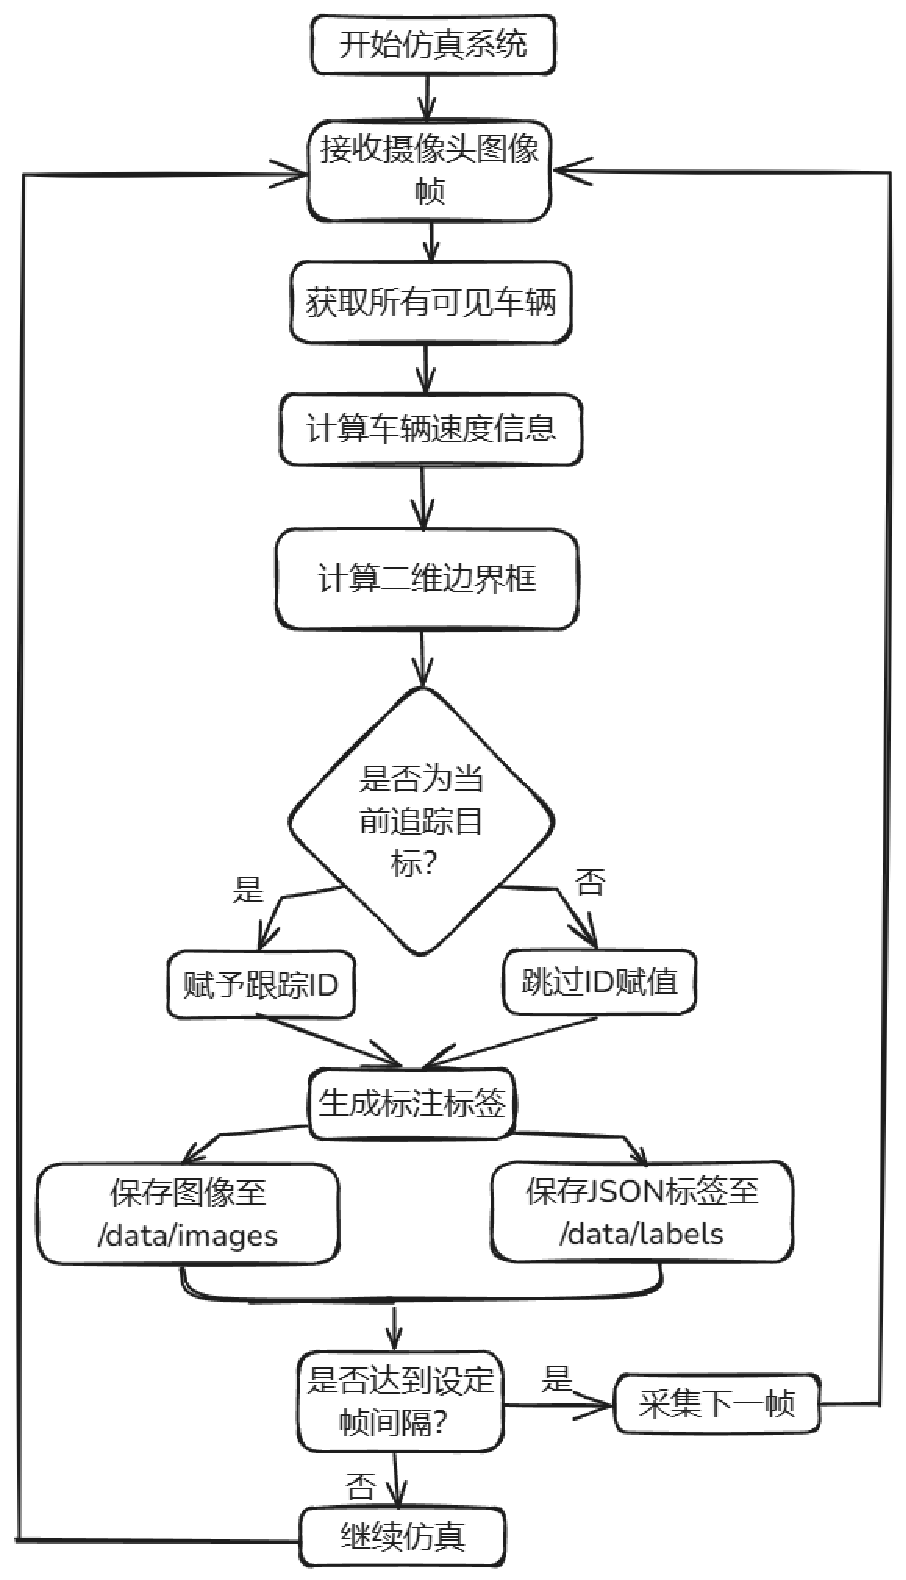
\includegraphics[width=0.8\textwidth]{images/图7 数据采集流程图.pdf}  % 引用转换后的 PDF 文件
    \caption{数据采集流程图}
    \label{fig:example_image}  % 可用于引用此图片
\end{figure}

\subsection{标注信息结构设计}

每个 JSON 标签文件对应一帧图像,包含该图像中所有检测到的车辆目标。标签信息以列表形式记录,每一项包含如下字段:

\textbf{bbox:}二维边界框左上角起 4 个顶点的图像坐标;

\textbf{speed\_m\_s:}目标瞬时速度(单位为米每秒);

\textbf{tracked\_id:}若目标被当前追踪模型识别并持续跟踪,则记录其分配 ID,否则为 null。

此结构可容纳常用目标检测框架(诸如YOLO,FasterR - CNN)以及跟踪框架(诸如DeepSORT,ByteTrack)所必要的数据格式,而且能够被拓展应用到行为分析任务里的时序建模当中。

\begin{figure}[H]
    \centering
    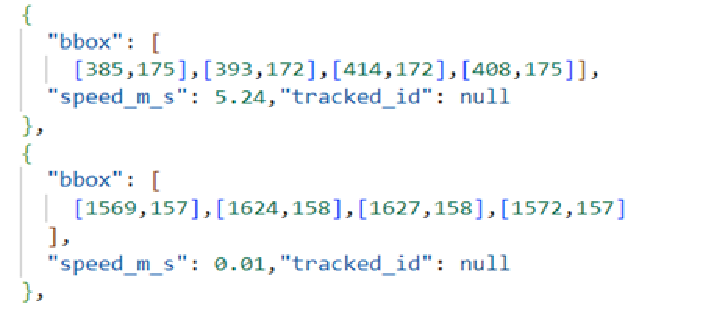
\includegraphics[width=0.8\textwidth]{images/图8 数据文件结构截图.pdf}  % 引用转换后的 PDF 文件
    \caption{数据文件结构截图}
    \label{fig:example_image}  % 可用于引用此图片
\end{figure}

\section{目标检测与跟踪模型设计}

\subsection{目标检测策略设计}

目标检测处于视觉感知系统的第一环,也是后面目标跟踪和意图分析的根基所在,要想加强整个系统的运行效率和鲁棒性,本文就在仿真环境里采用了一种依靠物理建模的投影式目标检测法,凭借Carla平台所供应的三维边界框以及车辆状态信息,避开了常规深度学习模型的推断流程,达成了一种既精准又快速的目标检测方案。

在 Carla 当中,每个交通参与者(涵盖车辆,行人,自行车等)被生成的时候都会带有自身的三维边界框信息(BoundingBox),参照图4-3可知,这个边界框由对象的局部中心点,长宽高(extent)以及朝向参数一起确定,准确地体现出目标物体所占据的空间范围。这些边界框是以局部坐标的形式存在的,必要通过变换才可以映射到图像平面上,详细来讲,系统先要得到目标的边界框顶点坐标,接着把它从局部坐标系转换成世界坐标,再依靠摄像头的变换矩阵投射到相机坐标系当中,最后用相机的内参实施二维图像平面的投影,从而形成目标在图像里的二维边界框。

\begin{figure}[H]
    \centering
    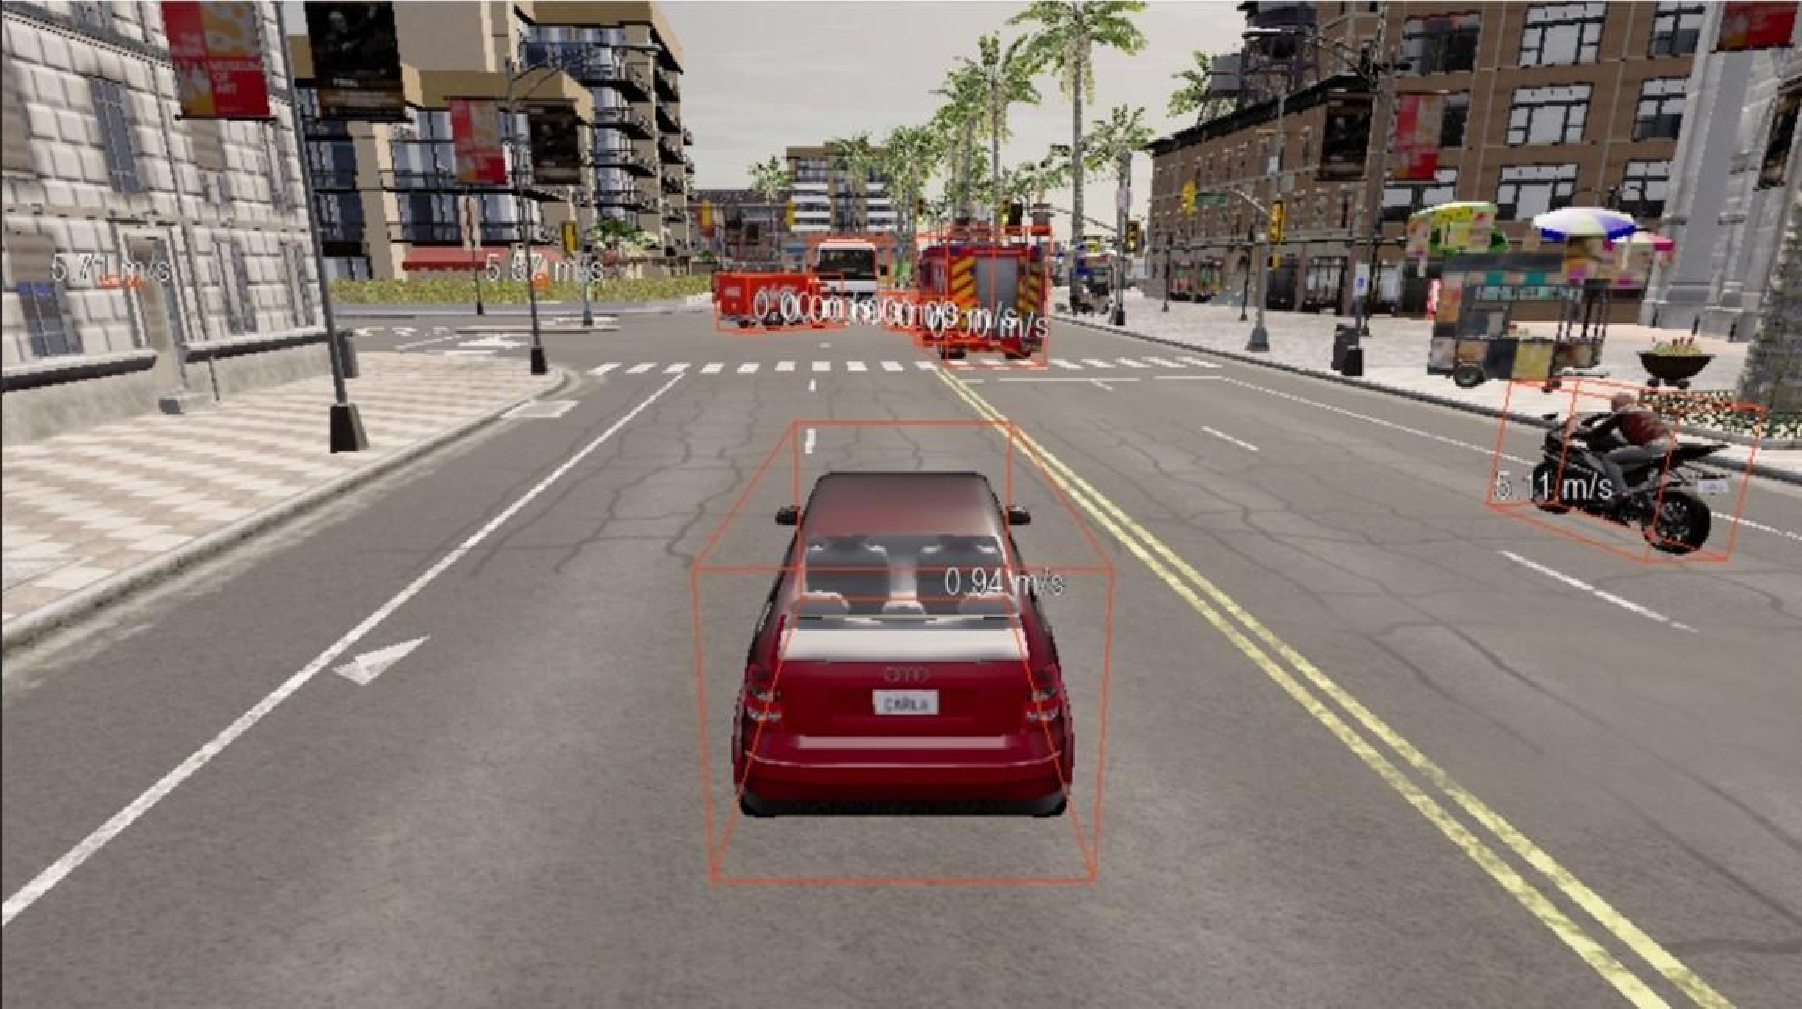
\includegraphics[width=0.8\textwidth]{images/图9 Bounding Box目标检测边界框示图.pdf}  % 引用转换后的 PDF 文件
    \caption{Bounding Box目标检测边界框示图}
    \label{fig:example_image}  % 可用于引用此图片
\end{figure}

此检测策略有不少优点,其一,依靠仿真物理参数而产生高精度检测,不会出现检测误差与误判情况;其二,其运算效率很高,检测时无需执行卷积操作或者获取繁杂的特征,从而大大削减了系统的负担;其三,这种检测结果蕴含着大量语义信息,诸如目标的速度,加速度,位置以及朝向等物理属性,给之后的行为分析给予了数据根基。而且,这种办法具有很强的可拓展性,可以针对不同类别的目标(比如车辆,行人)实施专门化处理并创建标签,还可以通过调整参数来自由把控采样频率和检测精度。

同依靠神经网络的端对端检测法(像YOLO,FasterR - CNN之类)比起来,本文所用的检测策略不用预先训练模型,也不要海量样本集,这样就明显减小了模型创建和布置的难度,而且,因为仿真环境具有确定性和可控性,所以这种方法有着较好的可重现性与一致性,可以用在自动驾驶系统前期研发期间的感知部件形成,算法证实以及功能考查等情形下。

总的来说,本文所设计的目标检测模块较好地发挥出Carla平台在高保真仿真上的长处,通过对三维边界框实施几何建模并向图像投影,形成起稳定,高效又具扩展性的二维目标检测机制,给后面的目标跟踪和意图识别模块赋予了有力的感知依托。


\subsection{DeepSORT 跟踪模型集成}

目标跟踪重点在于维持同一目标在连续帧里的身份,自动驾驶感知系统所处环境复杂且存在诸多干扰因素,目标也许会由于遮挡,加速,转弯等行为而出现大幅度的位置改变,所以创建起一种稳定又高效的视觉跟踪机制十分关键,依托此,本文借助DeepSORT算法塑造起单目标即时跟踪模块,并把它融合进Carla仿真平台当中的主控系统代码里面,从而达成了从检测输入一直到轨迹输出这样完整的功能流程。

相比于仅仅依靠位置信息的传统手段,DeepSORT即便处于遮挡环境之下仍然保留了一定的目标关联能力,本文所采用的是Python社区里相对更为成熟的deep\_sort\_realtime版本,其优势在于便于部署,接口清晰且适配性较好。

在整合环节当中,系统会把每帧通过Carla投影方式产生的二维检测框当作DeepSORT的输入,先对检测结果执行筛选(去掉那些面积太小,边界不正常的框),然后把它们全都统一格式化成[x,y,w,h]形式的矩形框输入列表,连同默认置信度,类别标签一道传给跟踪器。之后,DeepSORT内部利用卡尔曼滤波器去预估上一帧里全部跟踪目标此刻所处的位置,再融合新帧的检测框以及以往的运动轨迹,通过匈牙利算法来做目标之间的适配工作。 在匹配环节当中,DeepSORT并非仅仅依靠IOU(Intersection over Union)来做几何上的重叠度计算,其另外采用了通过卷积神经网络所得到的目标表观特征(ReID embedding),从而加强了对那些相似度极高的目标之间的辨别能力。

目标一旦匹配成功,便会被赋予独有的TrackID,其状态将会不断得到更新,而当检测器识别出未匹配上既有轨迹的新目标时,就会自动生成新的ID,进而产生一条新的跟踪轨迹。在本文所涉及的系统当中,由于是针对单目标展开跟踪设计的,所以只会把当前帧里距自车最近的那个目标选出来送进跟踪模块,如此一来便可以保障跟踪的唯一性与稳定性,此策略另外精简了系统的复杂程度,还能让后面意图分析环节更为方便地专门应对单个危险对象。

要做到视觉直观反馈,本文针对每帧图像利用pygame做即时绘制,把当下正在追踪的目标边界框用显眼的黄色矩形凸显出来,如下图4-4所示,并在框上面用文字表现这个目标的TrackID,系统也凭借颜色编码来区分不同状态,比如初始化,丢失,确认等等,从而优化人机交互的友好程度。

\begin{figure}[H]
    \centering
    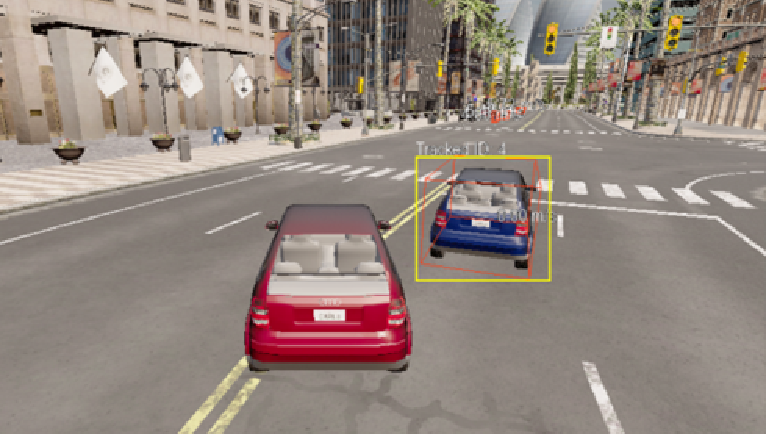
\includegraphics[width=0.8\textwidth]{images/图10 DeepSORT目标跟踪边界框示图.pdf}  % 引用转换后的 PDF 文件
    \caption{DeepSORT目标跟踪边界框示图}
    \label{fig:example_image}  % 可用于引用此图片
\end{figure}

从整体上看,DeepSORT模型在本系统中有较好的即时性与跟踪精准度,特别是在交通场景里发生遮挡,快速移动等状况的时候,依然可以守住目标轨迹的持续性和身份的一致性,这个跟踪单元既给后面的行为意图分析供应了稳固的输入根基,又为系统日后向多目标跟踪或者群体行为分析拓展构筑了技术架构根基。

\section{模型性能评估}

为了系统性地评估本文所构建的视觉目标检测与跟踪模块的性能,实验从处理效率与运行稳定性两个维度展开。性能评估基于 Carla 仿真平台,在 Town10 和 Town01 等典型城市场景中进行,所有实验均在本地 Windows 平台(CPU:Intel i7-10750F,GPU:NVIDIA RTX 2060,内存 16GB)执行,未启用 GPU 加速推理,测试结果具备代表性。

\subsection{系统帧处理时序分析}

图 4-5 展现了系统处理一帧图像数据时完整的流程及其各个阶段所耗费的时间,其中包含从仿真推进开始,通过图像获取,目标检测,目标跟踪,意图推断直到用户界面渲染结束这一整套过程,为精准度量性能,每个模块在主循环里设置了高精度计时器,用以记载时间戳,并算出相邻阶段之间所耗的时间,从而形成起帧处理的时序图。

\begin{figure}[H]
    \centering
    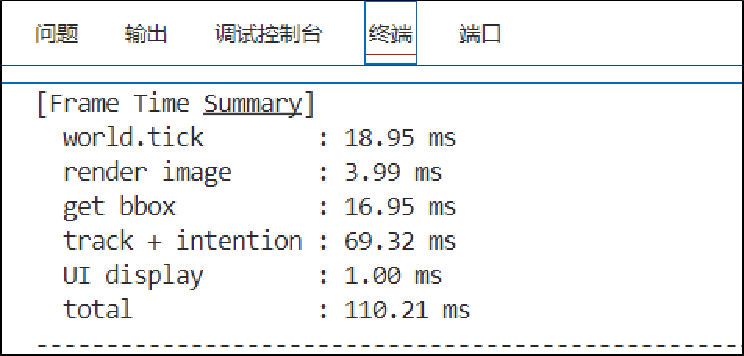
\includegraphics[width=0.8\textwidth]{images/图11 帧处理时序输出图.pdf}  % 引用转换后的 PDF 文件
    \caption{帧处理时序输出图}
    \label{fig:example_image}  % 可用于引用此图片
\end{figure}

将时序输出图转化成对应统计表格分析可知,单帧总处理时间为 110.21 毫秒,系统整体运行帧率约为 8.83 FPS,接近准实时运行性能要求。其中,各子模块平均耗时如下:

\begin{table}[htbp]
  \caption{模块时序统计表}
  \label{tab:timetable}
  \centering
  \begin{tabular}{lll}
    \toprule
    模块名称 & 平均耗时 & 比例估算 \\
    \midrule
    场景同步(tick) & 18.95ms & 17.2\% \\
    图像渲染(render) & 3.99ms & 3.6\% \\
    边界框生成(bbox) & 16.95ms & 15.4\% \\
    跟踪与意图分析 & 69.32ms & 62.9\% \\
    界面刷新(UI) & 1.00ms & 0.9\% \\
	总计(Total) & 110.21ms & 100\% \\
    \bottomrule
  \end{tabular}
\end{table}

场景同步(tick):平均时耗达到了5.98ms,其用途在于同Carla仿真服务器保持同步,并推动仿真世界向前迈进一帧,这一部分属于系统的基础性操作范畴,时耗较为稳定,基本上不会受到仿真地图复杂程度以及传感器数量之类因素的左右。

图像渲染(render):平均时耗达3.99ms,其职能在于把图像传感器所传回来的原始BGRA数据加以剖析,转换成RGB形式,再转变成pygame能够渲染的格式,从而交给后面的处理环节去做后续工作,这个阶段的性能比较稳定,属于图像类任务的一种常见开销。

边界框生成(bbox):平均时耗达11.97ms,利用Carla自身具备的3DBoundingBox投影功能,从真实车辆模型创建顶点坐标,并把这些坐标投影到摄像机图像平面上,这种做法取代了依靠图像的传统目标检测网络,明显减小了计算量,还改良了标注的准确性,给后续的跟踪供应了稳定的输入。

跟踪与意图分析(track + intention):这个模块所耗费的时间很多,达到了90.33ms,大约占据总帧处理时间的80\%,其过程包含DeepSORT的轨迹维持和状态更新(卡尔曼滤波,Hungarian符合,轨迹结合),还有依靠目标运动状态的意图判断逻辑(距离变化率,速度阈值,靠近风险判断等等),这个阶段耗时太多是影响帧率的关键因素,必要着重加以改善。

用户界面刷新(UI):平均耗费时间只有1.00ms,其功能在于把文字信息以及边界框显示到屏幕之上,这部分开销十分微小。

\subsection{模块耗时对比分析}

要想进一步明晰各个模块在资源占用上的相对贡献度,于是把连续100帧的平均耗时统计结果制成了柱状图(图4-6),从图上可以看出,DeepSORT跟踪模块以及意图推断阶段所占比例最大,这就表示,在以后的改良过程当中,应该最先考量针对这个模块展开算法提速或者模型压缩。

\begin{figure}[H]
    \centering
    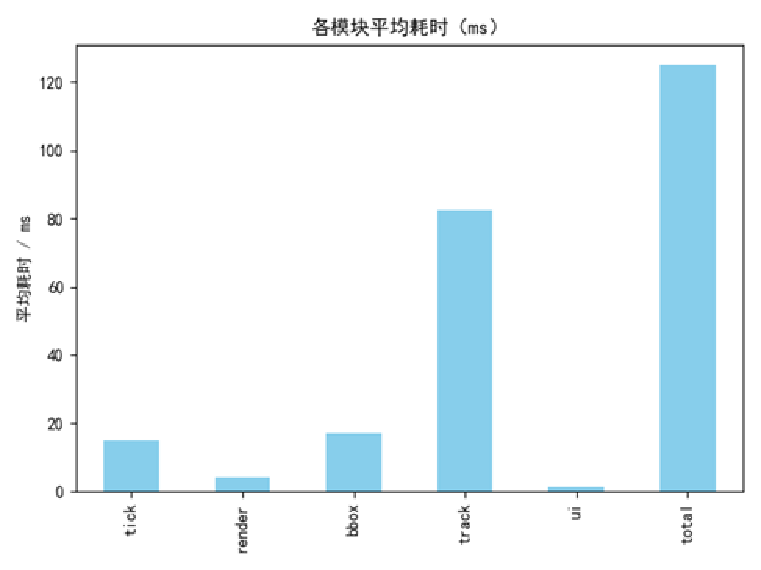
\includegraphics[width=0.8\textwidth]{images/图12 耗时统计柱状图.pdf}  % 引用转换后的 PDF 文件
    \caption{耗时统计柱状图}
    \label{fig:example_image}  % 可用于引用此图片
\end{figure}

可以看出,图像渲染、 边界框生成这类模块所耗费的时间比较少,这表明用Carla平台原本的三维boundingbox机制来取代图像检测模型是个有效的办法,既守住了高精度检测输入,又明显缩减了计算资源的占用量,界面渲染这个部分耗费的时间极少,可以在之后执行部署的时候关掉UI从而留出更多的处理能力。


\begin{tabular}{l l}
%  \verb|\songti| & {\songti 宋体} \\
%  \verb|\heiti| & {\heiti 黑体} \\
%   \verb|\kaiti| & {\kaiti 楷体}
\end{tabular}
